\documentclass[sigconf]{acmart}

\usepackage{booktabs} % For formal tables
\usepackage{wrapfig}
\usepackage{dblfloatfix}
\usepackage{hyperref}
\usepackage{balance}
\usepackage{colortbl}
\usepackage{cleveref}
\usepackage[shortlabels]{enumitem}
\usepackage[most]{tcolorbox}

\usepackage{pifont}% http://ctan.org/pkg/pifont

\newcommand{\cmark}{\ding{51}}%
\newcommand{\xmark}{\ding{55}}%

\newcommand{\bi}{\begin{itemize}[leftmargin=0.4cm]}
	\newcommand{\ei}{\end{itemize}}
\newcommand{\be}{\begin{enumerate}}
	\newcommand{\ee}{\end{enumerate}}


\makeatletter
\let\th@plain\relax
\makeatother


\definecolor{Gray}{gray}{0.85}
\usepackage{tikz}
\usepackage{framed}
\usepackage[framed]{ntheorem}
\usetikzlibrary{shadows}

\theoremclass{Lesson}
\theoremstyle{break}

% inner sep=10pt,
\tikzstyle{thmbox} = [rectangle, rounded corners, draw=black,
fill=Gray!40]
\newcommand\thmbox[1]{%
	\noindent\begin{tikzpicture}%
	\node [thmbox] (box){%
		\begin{minipage}{.94\textwidth}%
		\vspace{-0.1cm}#1\vspace{-0.1cm}%
		\end{minipage}%
	};%
	\end{tikzpicture}}

\let\theoremframecommand\thmbox
\newshadedtheorem{lesson}{Result}

\newcommand{\tion}[1]{{Section }\ref{sect:#1}}

\usepackage{listings}
\definecolor{MyDarkBlue}{rgb}{0,0.08,0.45} 
\lstset{
    language=Python,
    basicstyle=\sffamily\fontsize{2.5mm}{0.7em}\selectfont,
    breaklines=true,
    prebreak=\raisebox{0ex}[0ex][0ex]{\ensuremath{\hookleftarrow}},
    frame=l,
    keepspaces=false,
    showtabs=false,
    columns=fullflexible,
    showspaces=false,
    showstringspaces=false,
    keywordstyle=\bfseries\sffamily,
    emph={ m, r, k, frontier, cf, f, g, n}, emphstyle=\bfseries\color{blue!50!black},
    stringstyle=\color{green!50!black},
    commentstyle=\color{red!50!black}\it,
    numbers=left,
    captionpos=t,
    escapeinside={\%*}{*)}
}

% Copyright
%\setcopyright{none}
%\setcopyright{acmcopyright}
%\setcopyright{acmlicensed}
\setcopyright{rightsretained}
%\setcopyright{usgov}
%\setcopyright{usgovmixed}
%\setcopyright{cagov}
%\setcopyright{cagovmixed}


% DOI
\acmDOI{10.475/123_4}

% ISBN
\acmISBN{123-4567-24-567/08/06}

%Conference
\acmConference[WOODSTOCK'97]{ACM Woodstock conference}{July 1997}{El
  Paso, Texas USA} 
\acmYear{1997}
\copyrightyear{2016}


\acmArticle{4}
\acmPrice{15.00}

% These commands are optional
%\acmBooktitle{Transactions of the ACM Woodstock conference} 


\begin{document}
\title{700 Times Faster Than Deep Learning} 
\subtitle{A Case Study Comparing   Methods for Text Mining StackOverflow}


\author{Suvodeep Majumder, Nikhila Balaji, Katie Brey, Tim Menzies}  
\affiliation{%
  \institution{Computer Science, NC State, USA}
}
\email{smajumd3,nbalaji,kebrey@ncsu.edu}~~~\email{tim@menzies.us}

 
 

% The default list of authors is too long for headers.
\renewcommand{\shortauthors}{S. Majumder et al.}


\begin{abstract}
Deep learning is a representation-learning methods with multiple levels of representation, obtained by composing simple but non-linear modules that each transforms the representation at one level (starting with the raw input) into a representation at a higher, slightly more abstract level. Compared to the conventional machine learning algorithms, deep learning methods are very good at exploring high-dimensional data and is becoming widely used in many areas such as natural language processing, computer vision, image processing, text mining etc.. However, deep learners utilizes extensive computational power and can take a very long time to train. This makes it difficult to properly validate results, as well as for others to repeat results. For the problem of finding relatedness of Stack Overflow posts, it has been shown that a tuned SVM performs similarly to a deep learner, but is significantly faster to train. We extend this work to investigate the impact of local models. We first cluster the dataset and train tuned simple learners on each cluster in parallel. We show that this approach also performs similarly to the convolutional neural network, but is almost 965 times faster. This has significant implications for using global versus local models in  text mining problems. This paper tries to show the impact of learning time of model can be reduced greatly by creating local models without having impacts in model performance.
\end{abstract}

%
% The code below should be generated by the tool at
% http://dl.acm.org/ccs.cfm
% Please copy and paste the code instead of the example below. 
%
\begin{CCSXML}
<ccs2012>
 <concept>
  <concept_id>10010520.10010553.10010562</concept_id>
  <concept_desc>Computer systems organization~Embedded systems</concept_desc>
  <concept_significance>500</concept_significance>
 </concept>
 <concept>
  <concept_id>10010520.10010575.10010755</concept_id>
  <concept_desc>Computer systems organization~Redundancy</concept_desc>
  <concept_significance>300</concept_significance>
 </concept>
 <concept>
  <concept_id>10010520.10010553.10010554</concept_id>
  <concept_desc>Computer systems organization~Robotics</concept_desc>
  <concept_significance>100</concept_significance>
 </concept>
 <concept>
  <concept_id>10003033.10003083.10003095</concept_id>
  <concept_desc>Networks~Network reliability</concept_desc>
  <concept_significance>100</concept_significance>
 </concept>
</ccs2012>  
\end{CCSXML}

\ccsdesc[500]{Computer systems organization~Embedded systems}
\ccsdesc[300]{Computer systems organization~Redundancy}
\ccsdesc{Computer systems organization~Robotics}
\ccsdesc[100]{Networks~Network reliability}


\keywords{Deep learning, parameter tuning, DE, KNN, local versus global, k-means, SVM, CNN}


\maketitle

\section{Introduction}
    \label{sect:intro}
    Using deep learners like convolutional neural networks (CNN) has been a popular choice for text mining, since deep learning works well with high dimensional data [11]. Deep learners have been used to achieve impressive performance, but they are very expensive in terms of time and demand high computational resources.
    
    In this paper we build off of work done by Xu et al. ~\cite{xu2016predicting} and Fu et al. ~\cite{fu2017easy} on finding the semantic relatedness of Stack Overflow posts. A single stackoverflow question along with its complete answer is considered a knowledge unit (KU). If any two KUs are semantically related, they are considered as linkable knowledge. Otherwise, they are considered isolated. Linkable KUs can be broken down into three classes depending on how related they are scored. Xu first proposed the use of a CNN ~\cite{hubel1959receptive}, a specific kind of deep learner, that took 14 hours to train. Fu's work showed that a DE-tuned SVM performs similarly for this dataset, but trains 84x faster. One of the points Fu was trying to show was that the computational cost, resources and time that a state of the art learner demands can be avoided and similar performance results can be obtained if we replace the SOA learner with a simple standard learner like SVM and tune its parameters. 
    
    In this paper, we present our work, where we focus on the same idea that faster results can be obtained with standard learners - but we extend it further by building multiple local models and tries to show that local model can be built which has similar result, same as SOA learners, but can be trained fast. We propose to first cluster the data, and then run the tuned learners on each cluster in parallel. We tried this for both SVM (used by both Xu and Fu) and KNN - two combinations as seen below in table A. We compared this with two standard learners, KNN and SVM, and tuned versions of the same learners - a total of 4 more combinations. 
    
    Our study asks:
    \begin{itemize}
        \item 
            \textbf{RQ1}:  {\em Can we reproduce Fu’s results for tuning SVM with differential evolution (DE)?} 
            \begin{lesson}
                Yes, we found similar results.
            \end{lesson}
        \item 
            \textbf{RQ2}: {\em   How do the tuned local models compare with tuned and untuned global models in terms of performance and time?} 
            \begin{lesson}
                Local models perform comparably to their global model counterparts, but are significantly faster.
            \end{lesson}
        \item 
            \textbf{RQ3}: {\em   How does the performance of local models compare with global models and SOA models when used with SVM and KNN?} 
            \begin{lesson}  
                Local models worked between with SVM than with KNN.
            \end{lesson}
    \end{itemize}
    In summary, the contributions of this paper include:
    \begin{itemize}
        \item Offer local models as a technique to make learners context aware as well as significantly faster.
        \item Potentially present a faster method of text data classification than deep learning.
        \item Access to the code base - to reproduce, improve or refute our results.
    \end{itemize}
    \begin{table}[h!]
        \centering
        \begin{tabular}{c|c|p{4cm}}
            \textbf{Type} & \textbf{Abbreviation} & \textbf{Learner Description}\\
            \hline
            G & SVM & Support Vector Machine \\
            \hline
            G & KNN & K\-nearest Neighbors \\
            \hline
            G & KNN\_DE & K\-nearest Neighbors Tuned using differential evolution \\
            \hline
            G & SVM\_DE & Support Vector Machines Tuned using differential evolution \\
            \hline
            L & K\-Means\_KNN & Cluster + multiple KNNs \\
            \hline
            L & K\-Means\_DE\_KNN & Cluster + multiple KNNs tuned with DE \\
            \hline
            L & K\-Menas\_SVM & Cluster + multiple SVMs \\
            \hline
            L & K\-Means\_DE\_SVM & Cluster + multiple SVMs tuned with DE \\
            \hline
        \end{tabular}
        \caption{List of learner combinations in experiment}
        \label{tab:learners}
    \end{table}
    The rest of the paper is organized into the following sections
    \tion{Background and Motivation}provides background information  that directly relates to our research questions, in addition to laying out the motivation behind our work. In 
    \tion{experimentalSetup}a detailed description of our experimental setup and data, along with our performance criteria for evaluation is presented. It is followed by 
    \tion{result} the results of the experiments and answers to our research questions are detailed.
    \tion{threatsToValidity} discusses threats to validity. Finally 
    \tion{conclusion}concludes the paper with implications and scope for future work.
\section{Background and Motivation}
\label{sect: Background and Motivation}
    
    \subsection{Benefits of Local Models}
    \label{sssec:Benefits of Local Models}
    One benefit of building local models is that the learner is context aware. As per the "no free lunch" theorems ~\cite{wolpert1997no}, if an algorithm works well in one situation, there is another in which it doesn't. This tells us that learners perform differently on each dataset. But more than that, what if there are different regions in the data? Just like using the same learner on different datasets, using the same learner on every region of the data is not preferred. Ideally, a learner would be able to make different decisions for different regions of data.
    
    Time and CPU resources are other important factors to consider when using learners. Although today we have access to cloud resources to help with speeding up computationally-expensive tasks, the cost can be prohibitively expensive. This can make it hard for researchers to properly validate results, as well as for other researchers to repeat results. Resource cost needs to be more strongly considered when considering the tradeoffs of using particular learners.
    
    \subsection{SVM in Text Mining}
    \label{sssec:SVM in Text Mining}
    Support Vector Machine (SVM) is a type of supervised machine learning algorithm which analyzes data using classification or regression analysis. In SVM models the examples are points in space mapped in such a way that separate categories/classes are divided by as clear gap (plane or line) as possible. SVM ~\cite{suykens1999least} does this by transforming the original data space to a high dimensional space called feature space, and then uses hyper boundary to separate the classes/features.  
    
    Datasets in text mining can have a very large number of features. These features are relevant as they define the record/data point thoroughly and hence can't be thrown away. In most cases the document vectors are sparse and linearly separable. Because the learning capability of SVMs is independent of the dimensionality of the feature space ~\cite{joachims1998text}, it is very effective on text mining datasets.
    
    \subsection{KNN in Text Mining}
    \label{sssec:KNN in Text Mining}
    K-Nearest Neighbor ~\cite{zhang2007ml} (KNN)  is another type of supervised machine learning algorithm. It is a non-parametric ~\cite{goldberger2005neighbourhood} method used for classification and regression problems. Here K is the input and refers to the number of closest examples that the model will look for among the training data in the feature space. The output the model gives represents the class to which the test data belongs to and it depends on the majority vote of its k-nearest neighbor.
  
    KNN is one of the simplest types of machine learning algorithm to be used in text mining. A document is classified using the K nearest documents to it and then doing a majority vote in them, by using vector based distance method to calculate the similarity among the document matrices ~\cite{mihalcea2006corpus}.
    
    \subsection{Parameter Tuning with DE}
    \label{sssec:Parameter Tuning with DE}
    Differential Evolution (DE) is a stochastic population based optimization algorithm~\cite{storn1997differential}. DE starts with a frontier of candidate solution, then randomly select candidates from the frontier. Next, a new candidate solution is generated by extrapolating the selected candidates by a certain amount, if the probability of crossover is above a certain value. In our DE, we are using extrapolation amount as 0.75, the crossover probability as 0.3 and we are doing 60 repeats to find the best solution.
    
    We are using DE to tune the parameters of SVM and KNN. We are following the same procedure for Tuner that Fu cited in his paper that is based on Storn's differential evolution optimizer as shown in Figure~\ref{fig:pseudo_DE}.With SVM and KNN, Fu's tuner tries to maximize the objective score of the model based F1-score. as mentioned in Figure~\ref{fig:pseudo_DE}.
    
    \begin{figure}[!t]
    \small 
    \begin{lstlisting}[mathescape,linewidth=6.7cm,frame=none,numbers=right ]
      def DE( n=10, cf=0.3, f=0.7):  # default settings
        frontier = sets of guesses (n=10)
        best = frontier.1 # any value at all
        lives = 1
        while(lives$--$ > 0): 
          tmp = empty
          for i = 1 to $|$frontier$|$: # size of frontier
             old = frontier$_i$
             x,y,z = any three from frontier, picked at random
             new= copy(old)  
             for j = 1 to $|$new$|$: # for all attributes
               if rand() < cf    # at probability cf...
                  new.j = $x.j + f*(z.j - y.j)$  # ...change item j
             # end for
             new  = new if better(new,old) else old
             tmp$_i$ = new 
             if better(new,best) then
                best = new
                lives++ # enable one more generation
             end                  
          # end for
         frontier = tmp
        # end while
        return best
    \end{lstlisting} 
    \caption{Tuner Procedure - as mentioned in Fu\textquotesingle s paper. It is based on Storn\textquotesingle s DE optimizer.}
    \label{fig:pseudo_DE} 
    \vspace{-0.3cm}
    \end{figure}
    
    
    For SVM, we used the SVM module from Scikit-learn~\cite{pedregosa2011scikit}, a Python package for machine learning, where the parameters shown in Table~\ref{tab:DE_Parameters} are selected for tuning. Parameter C is to set the amount of regularization, which controls the tradeoff between the errors on training data and the model complexity. A small value for C will generate a simple model with more training errors, while a large value will lead to a complicated model with fewer errors. Kernel is to introduce different nonlinearities into the SVM model by applying kernel functions on the input data. Gamma defines how far the influence of a single training example reaches, with low values meaning 'far' and high values meaning 'close'. coef0 is an independent parameter used in sigmod and polynomial kernel function.
    
    Similarly KNN uses different parameters to control how it learns and how it predicts. For our experiment we have used KNN module from Scikit-learn, and the parameters in the table~\ref{tab:DE_Parameters} are selected for tuning the KNN. Parameter n\_neighbors is number of neighbors to be used for query to check and then use the classification based on majority vote ~\cite{guo2003knn}. Weight is another parameter which we are tuning, this parameter is used for prediction, it accepts value as 'uniform' where all the points in each neighborhood are weighted equally and other option in this is 'distance', here the weights are inverse of their distance from the new example so farther the point less weightage it has in deciding its class.
    
    \begin{table}[h!]
        \centering
        \begin{tabular}{c}
            SVM Tuning Parameters  \\
        \end{tabular}
        \begin{tabular}{p{1.5cm}|p{2cm}|p{4cm}}
            \textbf{Parameters} & \textbf{Tuning Range } & \textbf{Description} \\
            \hline
            C & [1,50] & Penalty parameter C of the error term \\
            \hline
            Kernal & ['liner', 'poly', 'rbf', 'sigmoid'] & Specify the kernel type to be used in the algorithms \\
            \hline
            gamma & [0,1] & Kernel coecient for 'rbf', 'poly' and 'sigmoid' \\
            \hline
            coef0 & [0,1] & Independent term in kernel function. It is only used in 'poly' and 'sigmoid' \\
            \hline
        \end{tabular} 
        \begin{tabular}{c}
            KNN Tuning Parameters  \\
        \end{tabular}
        \begin{tabular}{p{1.5cm}|p{2cm}|p{4cm}}
            \textbf{Parameters} & \textbf{Tuning Range } & \textbf{Description} \\
            \hline
            n\_neighbors & [2,10] & Number of neighbors \\
            \hline
            weights & ['uniform', 'distance'] & weight function using while prediction \\
            \hline
        \end{tabular}    
        \caption{'Tuning Range' of Parameters for SVM and KNN}
        \label{tab:DE_Parameters}
    \end{table}
    
    \subsection{Word Embedding}
    \label{sssec:Word Embedding}
    Word embedding is the process of converting words to vectors in order to compare their similarity. One method for doing this is Word2Vec, specifically the skip gram model, which is a two-layer neural network that converts words into semantic vector representations ~\cite{mikolov2013distributed}.
    
    In this paper, we use the word2vec models trained by Fu to convert the Stack Overflow text data into the corresponding vectors.

    \subsection{K-Means Clustering}
    \label{sssec:K-Means Clustering}
    K-means is an unsupervised learning machine learning algorithm that is used for clustering data ~\cite{jain2010data}. In k-means, k is an input that refers to the number of clusters the data set should be divided into. The algorithm initializes k number of centroids from the data and labels each as a cluster. For each data point it checks which centroid it is closest to, and assigns it to that cluster. After one pass to the data, centroids are recalculated and the process repeats until cluster stability is achieved. There are many parameters to control in k-means and there are multitude of ways to choose to customize these parameters. For instance, picking initial centroids, number of clusters, distance metric to compute point to centroid, number of iterations, criterion to stop the algorithm and so forth. In our experiments, we use the scikit-learn module -  sklearn.cluster.kMeans ~\cite{pedregosa2011scikit}. This method expects a k-value - or the number of initial centroids to supplied.
    \begin{wrapfigure}{r}{2in}\small
        \begin{lstlisting}[mathescape,linewidth=2in,frame=n,numbers=none]
        def GAP(training_data, nrefs=3, maxCluster = 15):
            gaps = gap in cluster
            for gap_index, k in enumerate(range(1, maxClusters)):
                for i in range(nrefs):
                    clf = KMeans(n_clusters=k, init='k-means++', max_iter=200, n_init=1)
                    clf.fit
                    inertia[i] = clf.inertia # calculate inertia of the model
                gaps[gap_index] = calculate diff in gap in new and original clusters
        return number of cluster
        \end{lstlisting} 
        \vspace{-0.2cm}
        \caption{Pseudocode of GAP Statistics}
        \label{fig:GAP_pseudocode} 
        \vspace{-0.3cm}
    \end{wrapfigure}
    Picking a k value for k-means is a challenge. If the k is smaller, we can have a model underfit that fails to capture any patterns in the data. On the other hand, if we had a very large k, we would be overfitting the model. The percent of variance explained will go up, but it is not capturing the bias in the data set. There are many theoretical ways to overcome this challenge and pick a sensible value for K. We used Gap statistics to determine the optimal number of k or centroids for our k-means ~\cite{mohajer2011comparison}~\cite{tibshirani2001estimating}. Gap statistic looks at the difference between the dispersion of the clustered data, and the dispersion of a null reference distribution, for increasing k values. It finds the largest k where the gap is bigger than the next gap minus a value that accounts for simulation error. Mathematically this is described as in figure~\ref{fig:GAP_pseudocode} ~\cite{tibshirani2001estimating}.

\section{Experimental Design}
\label{sect: Experimental Design}
    \subsection{Data}
    \label{sssec:Data}
    In our experiment, we use the same training and testing dataset as Xu ~\cite{xu2016predicting} and Fu ~\cite{fu2017easy}. Because we were not able to implement Xu\textquotesingle s CNN, we use the same datasets so that we can compare our results without introducing implementation bias. These datasets include 6,400 training examples and 1,600 testing examples. Each class is equally represented in both the training and test datasets, with 1600 of each class in the training dataset and 400 of each class in the test dataset, so no handling of class imbalance is necessary.
    
    Both test and training data are in pandas dataframe ~\cite{mckinney2011pandas} format, which includes a post Id, related post id, and a link type which is determined by a score between the 2 posts. The link between 2 posts can be of 4 types depending on the score between the sentences as per Table~\ref{tab:data_classl} - 
    
    \begin{table}[h!]
        \centering
        \begin{tabular}{c|c|c}
            \textbf{Scores} & \textbf{Class ID} & \textbf{Type} \\
            \hline
            1.0 & 1 & duplicate  \\
            \hline
            0.8 & 2 & direct link \\
            \hline
            0<x<0.8 & 3 & indirect link \\
            \hline
            0.00 & 4 & isolated \\
            \hline
        \end{tabular}
        \caption{Classification of data}
        \label{tab:data_classl}
    \end{table}
    
    For finding word embeddings ~\cite{mikolov2013distributed} of Stack Overflow ~\cite{barua2014developers} post data, we used the word2vec model trained by Fu. As per Fu\textquotesingle s paper, the word2vec model was created by randomly selecting 100,000 knowledge units tagged with "java" as the word corpus, preprocessing data as recommended by Xu, and then fitting the corpus into a python word2vec ~\cite{rehurek2010software} wrapper. To create a word embedding for each post, the word2vec model is used to create vector representations of each word, and then these vectors are averaged to get a vector for the entire document. Next, to get a vector representation of the pair of documents, the vector representations for each KU is then averaged. This is the value that is passed to the learners. The final data that is being passed to the learner is similar to Table~\ref{tab:data_format}
    
    \begin{table}[h!]
        \centering
        \begin{tabular}{p{.3cm}|p{1cm}|p{1cm}|p{1cm}|p{1cm}|p{1cm}|p{1cm}}
        \textbf{ID} & \textbf{Post Id} & \textbf{Related Post Id} & \textbf{Link Type Id} & \textbf{Post Id Vec} & \textbf{Related Post Id Vec} & \textbf{Output}  \\
        \hline
        0 & 283 & 297 & 1  & [...] & [...] & [...] \\
        \hline
        1 & 56 & 68 & 2  & [...] & [...] & [...] \\
        \hline
        2 & 5 & 16 & 3  & [...] & [...] & [...] \\
        \hline
        3 & 9083 & 6841 & 4  & [...] & [...] & [...] \\
        \hline
        \end{tabular}
        \caption{Training/Test data in pandas.dataframe format.}
        \label{tab:data_format}
    \end{table}
    
    \subsection{Method}
    \label{sssec:Method}
    Our proposed method is to build local models, in order to make learners context aware and decrease training time. To do this, we first cluster our data. Then we build a model for each cluster, parallelly. This process is shown in Figure~\ref{fig:our_model}.
    
    For our clustering algorithm we have used the K-Means algorithm from Scikit-learn. For the parameters, we used the k-means++ algorithm ~\cite{arthur2007k} for the initialization of cluster centroids, 200 maximum iterations, and 1 as the number of times the algorithm will run with different centroids. In order to choose K, the number of clusters, we used the GAP statistic method, discussed above.
    
    For each cluster, we build a learner that is tuned specifically for that cluster. We are looking at two different learners, SVM and KNN. As discussed above, to tune the learners, we are using DE, specifically Fu\textquotesingle s implementation. We are using f1-Score ~\cite{sokolova2006beyond} to evaluate the intermediate models in DE, as f1-score is calculated as the tradeoff between precision and recall. This will help us to get models which have both good precision and recall.
    
    \begin{figure}[!t]
    \small 
    \begin{lstlisting}[mathescape,linewidth=6.7cm,frame=none,numbers=right ]
      def KMeans( Word2Vec_model):  # The word2vec model for the Stack Overflow data
        train_data, test_data = Word2Vec.train_data, Word2Vec.test_data
        train_X, train_Y = train_data['Output'], train_data['LinkTypeID']
        queue = Queue()
        start = timer_start
        numCluster = GAP(train_X) #Getting best cluster number using GAP statistic
        clf = KMeans(n_cluster = numCluster, init='k-means++', max_iter=200, n_init=1)
        clf.fit(train_X) #training the KMeans to create Clusters
        train_data['clabels'] = clf.labels_
        target_model = SVM/KNN
        for l in range(numCluster):
            t = threading.Thread(target = target_model, args = [word2vec_src,cluster,queue,l]) # initializing threads for each cluster
            threads.append(t)
        for th in threads:
            th.start() #starting the threads
        for th in threads:
            svm_models.append(queue.get) #storing the models in a queue sent by the threads
        svm_model.sort() #sorting according to the order they were sent
        stop = timer_stop
        predicted['clabels'] = clf.predict(test_X)
        for i in range(svm_models[l])-1):
            for l in range(numClusters):
                cluster = predicted['clabels'] 
                svm_model = svm_models[l][i]
                cluster_X = cluster['Output']
                cluster_Y = cluster['LinkTypeId']
                total_cluster_Y = np.append(total_cluster_Y,cluster_Y)
                predicted_C = svm_model.predict(cluster_X)
                total_predicted = np.append(total_predicted,predicted_C)
            report_gen = metrics.classification_report(total_cluster_Y, total_predicted, labels=["1", "2", "3", "4"], digits=3)
        return time_taken = stop - start   
    \end{lstlisting} 
    \caption{Algorithm for creating the clusters and running the SVM/KNN on them}
    \label{fig:pseudo_KMeans} 
    \vspace{-0.3cm}
    \end{figure}
    
    To use the model, we first send the test data to K-means to find the cluster which it should belong to. Then we predict the class using that cluster\textquotesingle s learner.
    
    We have used a 10-fold cross validation ~\cite{kohavi1995study}, which was repeated 10 times for the training data. Thus, the results are the average of 100 models. Each learner (SVM or KNN) on each cluster has been trained on 90\% of the data from that cluster and tuned on rest of the 10\% and then tested on the untouched test data set. 
    
    \begin{figure}
        \centering
        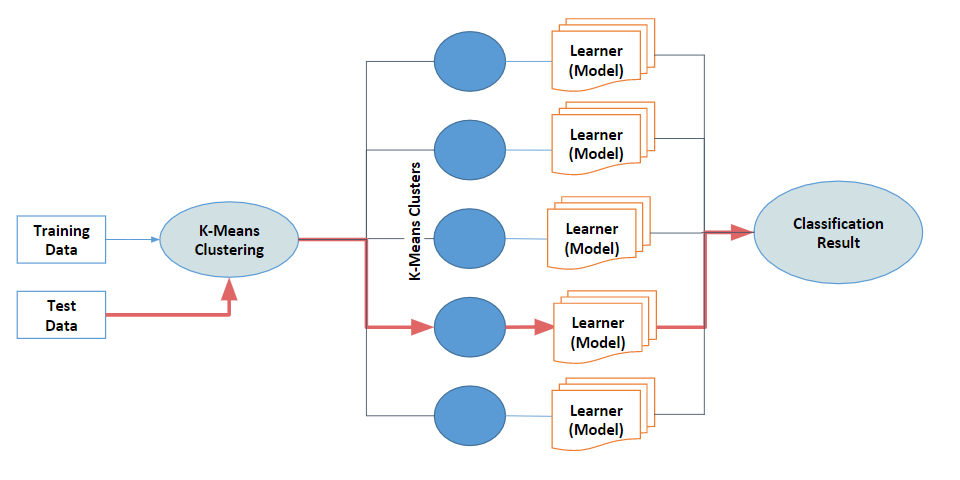
\includegraphics[width=\linewidth]{fig/Models.png}
        \caption{Model Architecture}
        \label{fig:our_model}
    \end{figure}
    
    \subsection{Performance Criteria}
    \label{sssec:performance_criteria}
    For evaluating our model, we collect and present the same metrics for performance evaluation as Xu and Fu, in order to compare results. These metrics are precision, recall and f1-score. In this multiclass classification problem we have 4 classes denoted as Duplicate(C1), Direct Link(C2), Indirect Link(C3) and Isolated(C4). In our results, we present class-wise metrics as well as the average for the whole model.
    
    \begin{table}[h!]
        \centering
        \begin{tabular}{c|c}
            & Predicted Class \\
            \hline
            Actual Class & \begin{tabular}{c|c|c|c|c}
                & C1  & C2  & C3  & C4  \\
                \hline
                C1 & C11 & C12 & C13 & C14 \\
                \hline
                C2 & C21 & C22 & C23 & C24 \\
                \hline
                C3 & C31 & C32 & C33 & C34 \\
                \hline
                C4 & C41 & C42 & C43 & C44 \\
            \end{tabular} \\
            \hline
        \end{tabular}
        \caption{Confusion Matrix}
        \label{tab:confusion_matrix}
    \end{table}
    
    Now from the confusion matrix describe above in Table~\ref{tab:confusion_matrix}, we can see the correct predictions are the one with label Cii for a class Ci. Now from this we will be able to calculate our evaluation matrixs. So here if a class Ci has been classified as Cj then it will be calculated as a wrong classification according to our confusion matrix.
    
    So from the confusion matrix we can calculate the precision, recall and F-Score as follows
    
    \begin{equation}
        precision = \frac{C_i_i}{\sum\limits_{i}C_i_j}
    \end{equation}
        \begin{equation}
        recall = \frac{C_i_i}{\sum\limits_{i}C_j_i}
    \end{equation}
        \begin{equation}
        F-Score = \frac{2*recall*precision}{(precision + recall)}
    \end{equation}

    \subsection{Statistical Analysis}
    \label{sssec:Statistical Analysis}
    In order to compare results of our local models with other models, there are two useful tests: significance tests ~\cite{bentler1980significance} and effect size tests ~\cite{rosenthal1994parametric}~\cite{chen2002correlation}. Whereas significance tests tell statistically whether results are distinct enough to be considered different, effect size tells us whether that difference is actually interesting. In order to determine whether the difference in performance of different methods is significant, we use the Scott-Knott, which ranks treatments using a recursive bi-clustering algorithm. At each level, treatments are split where expected value of the treatments has most changed from before. Results in each rank are considered the same according to both significance and effect size tests. Specifically, our Scott-Knott uses the nonparametric bootstrap ~\cite{efron1982jackknife} method and A12 test.
    

\section{Results}
\label{sect:Result}
    In this section we try to answer the research questions that we have asked as per our experiment. This includes all of our experiment results along with our take on that. 
    
    So as part of the experiment we tried to compare the result of Fu\textquotesingle s DE SVM with our clustered with DE SVM  and clusterer then DE KNN. And we also compared the result with XU\textquotesingle s CNN with our models. 
    
    \textbf{RQ1}:  {\em Can we reproduce Fu\textquotesingle s results for tuning SVM with differential evolution (DE)?}
    
    Our first task as part of this experiment was to recreate Fu\textquotesingle s work so that we have a baseline to measure against. We used the same SVM from Scikit-learn with the parameters tuned as mentioned in Table~\ref{tab:DE_Parameters}. We also compared the training time of our DE+SVM model to compare it with Fu\textquotesingle s model. Table~\ref{tab:performance Measure comp} below shows the class by class comparison for all the performance measure we are using.
    
    From Table~\ref{tab:performance Measure comp} and Figure~\ref{fig:delta_comp_Fu's_ours} we can say that the model we have used SVM with DE for hyperparameter tuning ~\cite{duan2003evaluation}~\cite{fu2017easy} is similar to what Fu has used in his paper. We see from this figure that for most of the cases apart from class 3, our model has performed a little better, but the delta between the performance is very small to consider. So to answer RQ1, we have successfully implemented Fu\textquotesingle s SVM and seeing the results we can say we will be able to use this implementation to compare our results and use this version of DE+SVM implementation~\cite{fu2017easy} for our next part experiment.
        \begin{table}
        \centering
        \begin{tabular}{c|p{2cm}|p{2cm}|p{2cm}}
            Class & Precision Avg & Recall Avg & F-Score Avg \\
            \hline
            C1 & \begin{tabular}{c|c}
                0.910  & 0.885 \\
             \end{tabular} & \begin{tabular}{c|c}
                0.924  & 0.860 \\
             \end{tabular}  & \begin{tabular}{c|c}
                0.917  & 0.878 \\
             \end{tabular}\\
            \hline
            C2 & \begin{tabular}{c|c}
                0.918  & 0.851 \\
             \end{tabular} & \begin{tabular}{c|c}
                0.907  & 0.828 \\
             \end{tabular}  & \begin{tabular}{c|c}
                0.910  & 0.841 \\
             \end{tabular}\\
            \hline
            C3 & \begin{tabular}{c|c}
                0.971  & 0.994 \\
             \end{tabular} & \begin{tabular}{c|c}
                0.992  & 0.995 \\
             \end{tabular}  & \begin{tabular}{c|c}
                0.981  & 0.969 \\
             \end{tabular}\\
            \hline
            C4 & \begin{tabular}{c|c}
                0.943  & 0.903 \\
             \end{tabular} & \begin{tabular}{c|c}
                0.925  & 0.905 \\
             \end{tabular}  & \begin{tabular}{c|c}
                0.934  & 0.909 \\
             \end{tabular}\\
            \hline
            Overall & \begin{tabular}{c|c}
                0.936  & 0.908 \\
             \end{tabular} & \begin{tabular}{c|c}
                0.936  & 0.897 \\
             \end{tabular}  & \begin{tabular}{c|c}
                0.935  & 0.899 \\
             \end{tabular}\\
        \end{tabular}
        \caption{Comparison of all performance measure between Our DE\_SVM and Fu\textquotesingle s DE\_SVM }
        \label{tab:performance Measure comp}
    \end{table}
    
    \begin{figure}
        \centering
        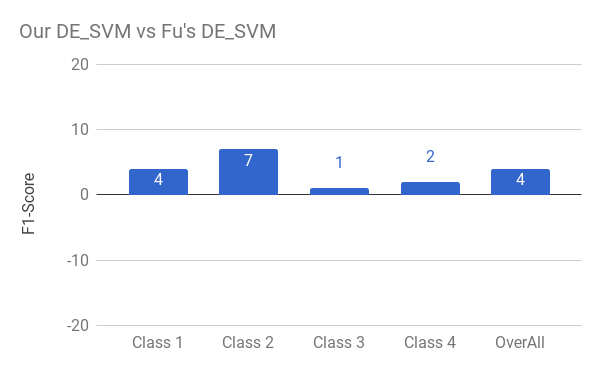
\includegraphics[width=\linewidth]{fig/delta_chart_our_SVM_DE_vs_FU's_SVM_DE.png}
        \caption{Score Delta between our DE\_SVM with Fu\textquotesingle s DE\_SVM. Positive values indicate when our SVM performs better than Fu\textquotesingle s.}
        \label{fig:delta_comp_Fu's_ours}
    \end{figure}
    
    \textbf{RQ2}: {\em   How do the tuned local models compare with tuned and untuned global models in terms of performance and time?}
    
    For this part of the experiment, we evaluated our method. As discussed above, we have used Gap statistic~\cite{mohajer2011comparison}~\cite{tibshirani2001estimating} for finding the best number of clusters, using minimum and maximum number of clusters as 3 and 15, respectively. As part of our experiment we are normally getting 13 clusters for the training dataset. 
    
    Now for the next part of the experiment we have to create the classifiers on each of the clusters. For us we have used SVM, KNN and both of the algorithms with DE-tuned parameter. For the normal SVM and KNN we have used the default parameters, described in Table 2. For performing the DE on the learners, we have used the parameters defined in Table 2. 
    
    We measured the time taken for this model to train which includes time taken by GAP statistic, K-Means training time, and SVM/KNN with DE training time.
    
    We are comparing the results with Fu\textquotesingle s SVM, and XU\textquotesingle s CNN with our models. From the Figure~\ref{fig:time} we can see when we cluster data and then create local models on each cluster we are seeing good performance improvement. In the case of K-Means then DE with SVM we are seeing 14 times improvement from using SVM with DE. And almost 965x improvement in training time from XU\textquotesingle s CNN. With K-Means then DE with KNN, we see around 11x performance improvement and from XU\textquotesingle s CNN the improvement is around 700x. Seeing these results we can answer our 2nd question that local models do in fact reduce the runtime by many folds.
    
    \begin{figure}
        \centering
        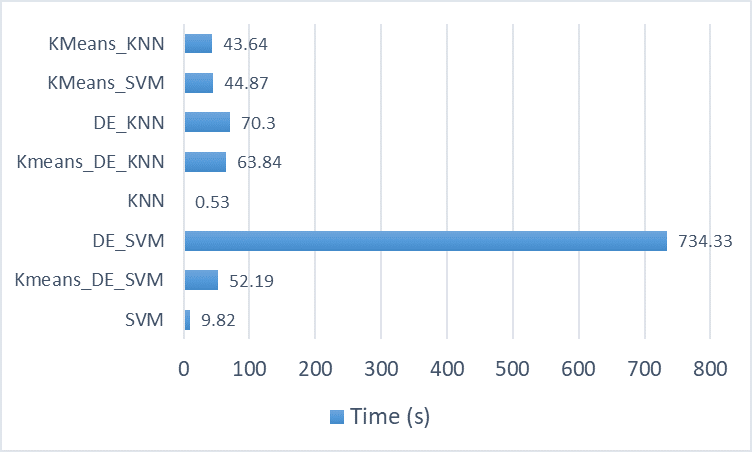
\includegraphics[width=\linewidth]{fig/Time.png}
        \caption{Training Time Comparison between models}
        \label{fig:time}
    \end{figure}
    
    \textbf{RQ3}: {\em   How does the performance of local models compare with global models and SOA models when used with SVM and KNN?} 
    
    \begin{figure}
        \centering
        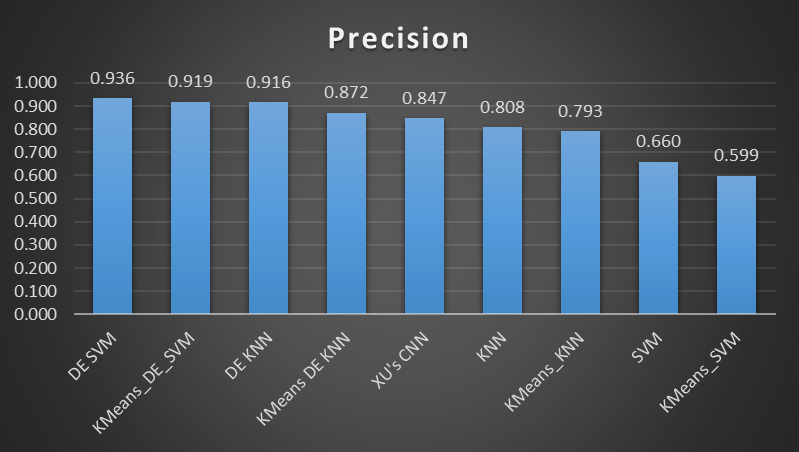
\includegraphics[width=\linewidth]{fig/precision.png}
        \caption{Precision Score for all learners}
        \label{fig:precison}
    \end{figure}
    
    The final part of our research question was to check if the local models performance is comparable to Fu's DE\_SVM and the XU's SOA CNN. To evaluate the performance of the models we are comparing performance measures described in Section~\ref{sssec:performance_criteria}. As mentioned in the section, we have done a 10 fold - 10 repeat cross validation, so all the results are average of 100 models created. 
    
    The 1st performance measure is precision is in Figure~\ref{fig:precison}. The precision of 9 learners discussed in Table~\ref{tab:my_label}, for overall class performance is shown in the figure. Now By evaluating the table we can see DE\_SVM's precsion is at 0.936 followed by KMeans\_DE\_SVM at 0.919. Similarly DE\_KNN is followed by KMeans\_DE\_KNN. Both the local models performance almost similar to the global models. But both the models out-performs XU's CNN. Similar trend is also noticeable between without DE versions of the algorithms with default parameters.
    
     \begin{figure}
        \centering
        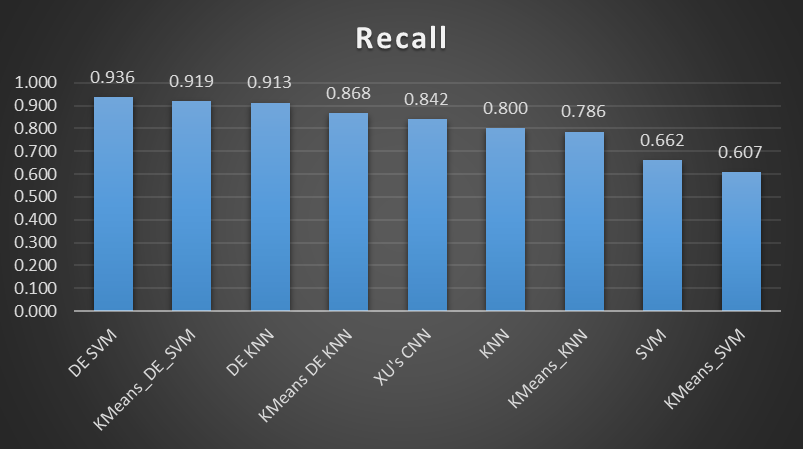
\includegraphics[width=\linewidth]{fig/recall.png}
        \caption{Recall score for all learners}
        \label{fig:Recall}
    \end{figure}
    
    In Figure~\ref{fig:Recall} we see the performance measures of all the models in similar way for recall. In here as well we see similar results as precision, global and local models with parameter tuning performs almost similar, but out-performs CNN.
    
    \begin{figure}
        \centering
        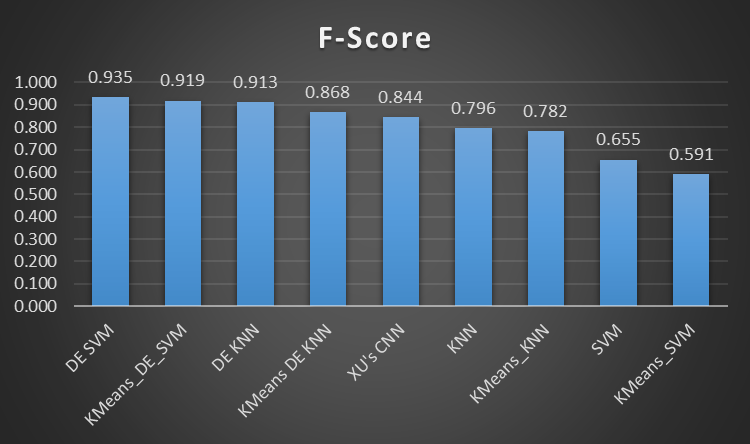
\includegraphics[width=\linewidth]{fig/f-score.png}
        \caption{F1-Score comparison for all learners}
        \label{fig:F1-Score}
    \end{figure}
    
    Figure~\ref{fig:F1-Score} for F-Score measure which is a better understanding of the trade off between precision and recall. Here as well we see similar result.
    
    Seeing these results it was assumable that from overall performance evaluation local models performance is almost similar to it's global version. But we wanted to make delta comparison between class performance of all the performance criteria for local vs global models for SVM and KNN, and also XU's CNN vs local models. Figure~\ref{fig:Global_vs_Local_DE_SVM} shows the class wise score delta between local KMeans\_DE\_SVM vs global DE\_SVM. We see from the Figure~\ref{fig:Global_vs_Local_DE_SVM} that for all performance criteria and all the classes, the global model performs a slightly better, but the delta is very low.
    
    Figure~\ref{fig:CNN_vs_KMeans_DE_SVM} shows the score delta between XU's CNN and local KMeans\_DE\_SVM. We see in the result that except class 2 recall our models performs better and the delta score is high in class 3 and 4.

    \begin{figure}
        \centering
        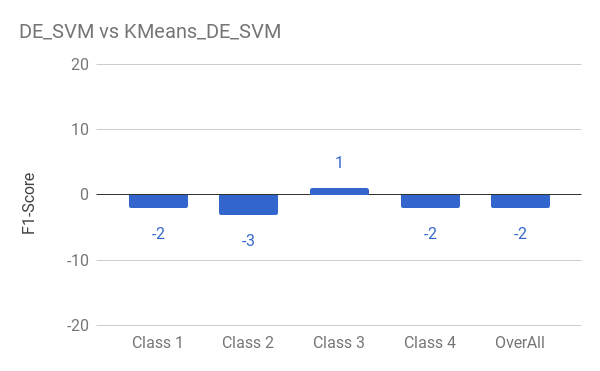
\includegraphics[width=\linewidth]{fig/de_vs_KMenas.png}
        \caption{Class wise Score Delta between Global DE\_SVM vs Local KMeans\_DE\_SVM}
        \label{fig:Global_vs_Local_DE_SVM}
    \end{figure}
    
    \begin{figure}
        \centering
        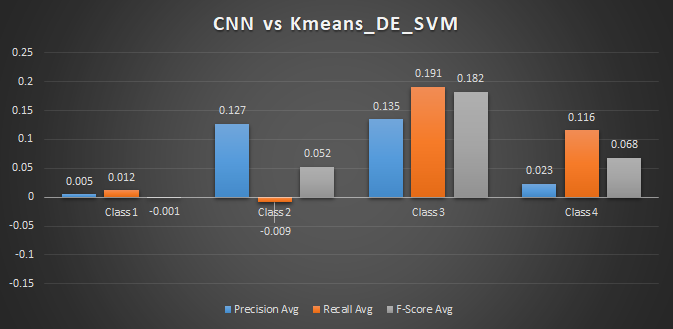
\includegraphics[width=\linewidth]{fig/cnn_vs_Kmeans.png}
        \caption{Class wise score delta between XU's CNN and Local KMeans\_DE\_SVM}
        \label{fig:CNN_vs_KMeans_DE_SVM}
    \end{figure}
    
    Next we see in Figure~\ref{fig:Global_vs_Local_DE_KNN} class wise score delta of performance matrices between local KMeans\_DE\_KNN vs global DE\_KNN, and we can see similar result as of the global and local SVM version. in most of the cases the global model's performance is slightly better than local model. In case of XU's CNN vs local KMeans\_DE\_KNN model we see that for class 3 the performance increase is very noticeable for rest of the classes and performance measure the results are almost similar, which we can notice in Figure~\ref{fig:CNN_vs_KMeans_DE_KNN}.
    
    \begin{figure}
        \centering
        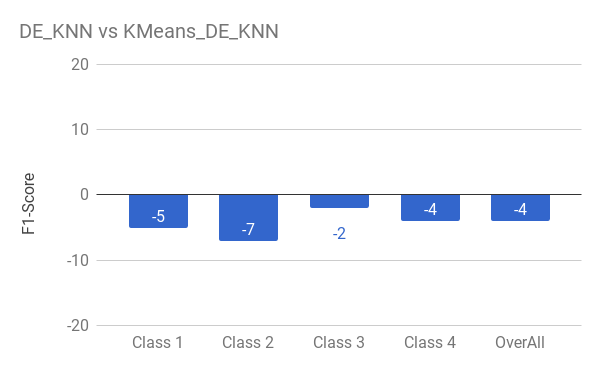
\includegraphics[width=\linewidth]{fig/KNN_vs_KMeans.png}
        \caption{Class wise score delta between Global DE\_KNN vs Local KMeans\_DE\_KNN}
        \label{fig:Global_vs_Local_DE_KNN}
    \end{figure}
    
    \begin{figure}
        \centering
        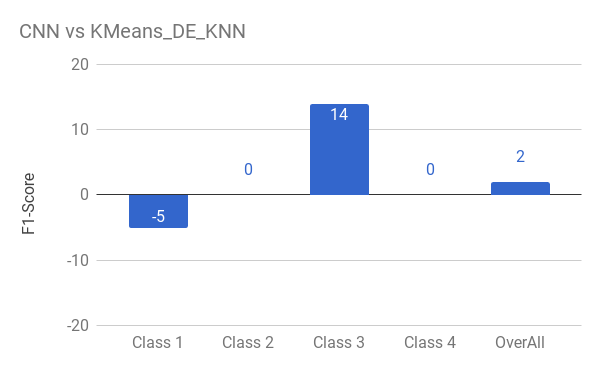
\includegraphics[width=\linewidth]{fig/cnn_vs_Kmeans_Knn.png}
        \caption{Class wise score delta between XU's CNN and Local KMeans\_DE\_SVM}
        \label{fig:CNN_vs_KMeans_DE_KNN}
    \end{figure}
    
    Seeing all the results we can see there is a little difference between the global vs local models as well a difference between SOA CNN and local models. But we see in the score delta charts the difference is very small most if time. We wanted to check if these performance measure difference is statistically significant or not. So we ranked the models using scott-knott test as mentioned in Section~\ref{sssec:Statistical Analysis}. The test was conducted on all the performance measures separately with all the results from 10 fold - 10 repeat validations.
    
    \begin{figure}
        \centering
        \tcbox[sharp corners, boxsep=1mm, boxrule=0.5mm, 
            colframe=blue!30!black, colback=white]{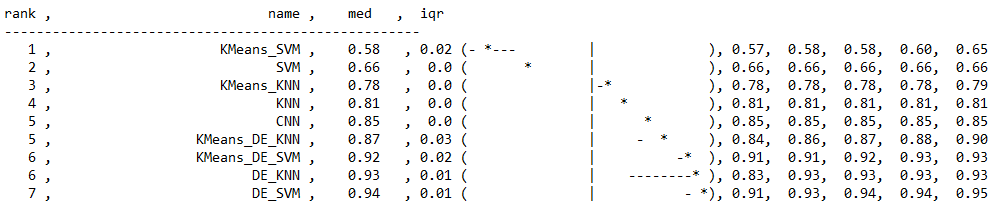
\includegraphics[width=\linewidth]{fig/precision_st.png}}
        \caption{Scott-Knott ranking for Precision}
        \label{fig:Scott-Knott ranking for Precision}
    \end{figure}
    
    \begin{figure}
        \centering
        \tcbox[sharp corners, boxsep=1mm, boxrule=0.5mm, 
            colframe=blue!30!black, colback=white]{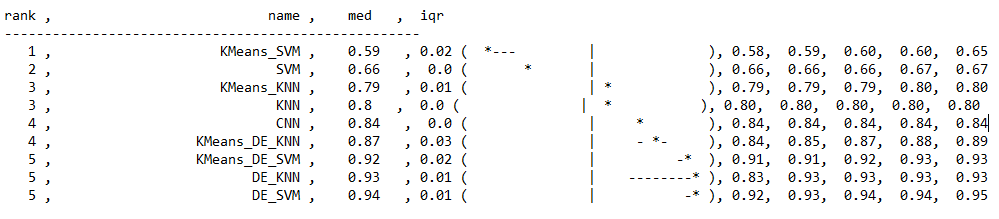
\includegraphics[width=\linewidth]{fig/recall_st.png}}
        \caption{Scott-Knott ranking for Recall}
        \label{fig:Scott-Knott ranking for Recall}
    \end{figure}
    
    \begin{figure}
        \centering
        \tcbox[sharp corners, boxsep=1mm, boxrule=0.5mm, 
            colframe=blue!30!black, colback=white]{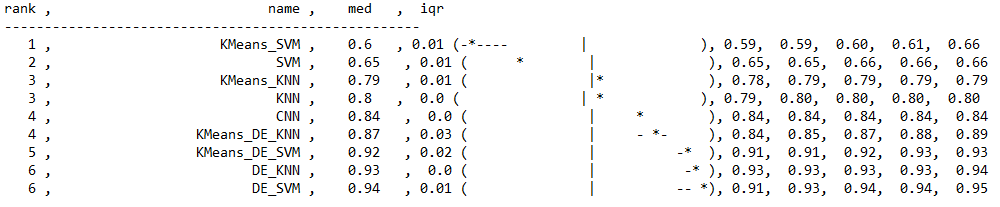
\includegraphics[width=\linewidth]{fig/f-score_st.png}}
        \caption{Scott-Knott ranking for F-Score}
        \label{fig:Scott-Knott ranking for F-Score}
    \end{figure}

    From the results of the Scott-Knott test we can see that in case of precision the DE\_SVM and KMeans\_DE\_SVM have separate ranking as 6 for  KMeans\_DE\_SVM and 7 for DE\_SVM and as well XU's CNN is at rank 5. So in case of precision we can say the results of these 3 models are statistically different, but looking at the median we can say although they are different they have very similar or we can say comparable results. We see in Figure~\ref{fig:Scott-Knott ranking for Recall} DE\_SVM and KMeans\_DE\_SVM are ranked similar, so in case of recall their performance is statistically same, both ranked at 5, while XU's CNN is ranked at 4. And the results are similar in case of F-Score as seen in Figure~\ref{fig:Scott-Knott ranking for F-Score}, with DE\_SVM ranked at 6 and KMeans\_DE\_SVM ranked at 5 and XU's CNN ranked at 4.
    
    So seeing all the results of difference perfromance measures and ranking test that although local models have a slightly lower measure than global models in case of precision and f-score and a slightly better performance in recall, overall the local models performs almost similar to their global part and the models performance is comparable to state of the art convolution neural networks.
    
    
\section{THREATS TO VALIDITY}
\label{sect:THREATS TO VALIDITY}
    Threats to internal validity of our work includes the fact that we started our experiment directly based on the code repository that was provided in the "Easy Over Hard" paper. Since we forked Fu's GitHub Repo link and collected the metrics for DE\_SVM that  our results validity are directly linked to the validity of his results. In order to continue with the other learners described in Table~\ref{tab:learners}, we added additional code and scripts to their code base . In the "Easy Over Hard" paper, Fu also points out that since the original Word Embedding + SVM baseline method was not available publicly, he implemented his own version and got results very similar to the ones reported on Xu's study. 
    
    In our paper, the performance metrics we report for our experiments - recall, precision, f1-score, and accuracy - are the same ones reported on Fu's DE\_SVM paper and the XU's CNN  paper. The experimental results for our learner combination in Table A are very much comparable to the DE\_SVM results. The reason we tried building local models using cluster-first approach was to capture any local similarities or properties that the data domain might have. It worked out well in our case, but that does not mean that other external text mining datasets will have any local patterns that can be captured. It might be the case there are not any locally specific characteristics and hence global models with tuned standard learners might produce similar results as local models. But it is very much possible that there might be local nuances in the dataset that can be well captured by the clusters and hence the models trained on the subsets might be better at prediction.


\section{CONCLUSION}
\label{sect:CONCLUSION}
    From our work, we found that applying local models can significantly speed up the training time. They do not appear to improve performance, however. We were able achieve comparable performance to a deep learner in significantly less time.
    
    We would like to highlight the importance of "No Free Lunch Theorem" ~\cite{wolpert1997no} in machine learning. Just because our cluster-first method works well with this data, it does not mean it is always going to perform equally well on all other text mining applications. No learner or set of learners is a perfect solution in all situations. Hence, it is very important to try and explore the problem domain with different learners before concluding what is the best solution to solve a problem. Exploring and trying out standard learners with minor adaptations can provide more insight or good enough performance, before investing in deep learners. 
    
    For future work, we suggest trying several variations of this experiment that may have interesting results. In our experiment we clustered pairs of Stack Overflow posts. However, it might make more sense to cluster posts individually, to group posts together before making finer-tuned decisions on whether they are related. Another question we would like to look at is whether there is a dependency between the number of clusters chosen and the tuned learner. Instead of tuning the learner separately from the clustering algorithm, what if we tuned the system as a whole? 


\bibliographystyle{ACM-Reference-Format}
\bibliography{700faster} 

\end{document}